%%
%% This is file `pst-pdf-example2.tex',
%% generated with the docstrip utility.
%%
%% The original source files were:
%%
%% pst-pdf.dtx  (with options: `example2')
%% 
%% This is a generated file.
%% 
%% Copyright (C) 2004-2008 by Rolf Niepraschk <Rolf.Niepraschk@gmx.de>
%%                            and Hubert Gaesslein
%% 
%% This file may be distributed and/or modified under the conditions of
%% the LaTeX Project Public License, either version 1.2 of this license
%% or (at your option) any later version.  The latest version of this
%% license is in:
%% 
%%    http://www.latex-project.org/lppl.txt
%% 
%% and version 1.2 or later is part of all distributions of LaTeX version
%% 1999/12/01 or later.
%% 
%% Process this file with the scripts `ps4pdf' or `ps4pdf.bat' or call
%%
%%   latex pst-pdf-example2.tex
%%   dvips -Ppdf -o pst-pdf-example2-pics.ps pst-pdf-example2.dvi
%%   ps2pdf -dAutoRotatePages=/None pst-pdf-example2-pics.ps pst-pdf-example2-pics.pdf
%%   pdflatex pst-pdf-example2.tex
%%
\listfiles\errorcontextlines=100\relax
\documentclass[12pt]{article}

%% before `psfrag'!
\usepackage[displaymath,dvipsnames]{pst-pdf}
%%\usepackage[displaymath,dvipsnames,notightpage]{pst-pdf}

\usepackage{pst-node,pst-tree}

\usepackage{psfrag,tabularx}

\pagestyle{empty}

\begin{postscript}[trim=0 0 0 0,ignore]
  
\includegraphics[width=.475\textwidth]{penguin.eps}
\end{postscript}
\savepicture{ps:A}

\begin{pst-pdf-defs}%

%% This definition must be within the pst-pdf-defs environment!
\newcommand*\mytree{%
  \begin{psmatrix}[rowsep=.2cm,colsep=2cm]
               &       & E   \\
               & A     &     \\
               &       & F   \\
  $\bullet$    &       &     \\
               &       & G   \\
               & B     &     \\
               &       & H   \\
  \scriptsize
  \psset{shortput=nab,arrows=->,labelsep=2pt,nodesep=2pt,nrot=:U}

  \ncline{4,1}{2,2}\ncput*{$0,2$}
  \ncline{4,1}{6,2}\ncput*{$x$}

  \ncline{2,2}{1,3}\ncput*{$0,3$}
  \ncline{2,2}{3,3}\ncput*{$y$}

  \ncline{6,2}{5,3}\ncput*{$z$}
  \ncline{6,2}{7,3}\ncput*{$0,8$}
  \end{psmatrix}%
}

\end{pst-pdf-defs}%

%% This works without the pst-pdf-defs environment!
\newcommand*\mymatrix{%
  \begin{postscript}
  \[
  \begin{array}{rcl}
   a & b & c \\
   1 & 2 & 3 \\
  \end{array}
  \]
  \end{postscript}%
}

\begin{document}

\setkeys{Gin}{showname,frame}%

\psset{unit=0.0714\textwidth}% 1/14 * \textwidth
\newpsobject{showgrid}{psgrid}{subgriddiv=1,griddots=10,gridlabels=6pt}

\newcommand*\BASEMARKER{\rule{.5em}{.4pt}}

\setlength\parindent{0pt}

\centering

\section*{\textsf{pst-pdf:}
  PSTricks and other PostScript code in pdf\LaTeX\ documents}

\vfill

\begin{pspicture}(-5.5,-5.25)(5.25,5.25)%
%%\begin{pspicture}[trim=-.5 -.25 .25 .25,frame](-5,-5)(5,5)% PSTricks2
  \pscircle*[linecolor=Apricot]{5}
  \rput(0,0.5){
\includegraphics[width=8\psxunit]{elephant}}
  \Huge\sffamily\bfseries
  \rput(-4.5,4.5){A} \rput(4.5,4.5){B}
  \rput(-4.5,-4.5){C}\rput(4.5,-4.5){D}
  \rmfamily
  \rput(0,-3.8){PSTricks}
  \rput(0,3.8){\LaTeX}
  \showgrid
\end{pspicture}\savepicture{ps:B}

\vfill\null\newpage

\usepicture{ps:A}
\hfill
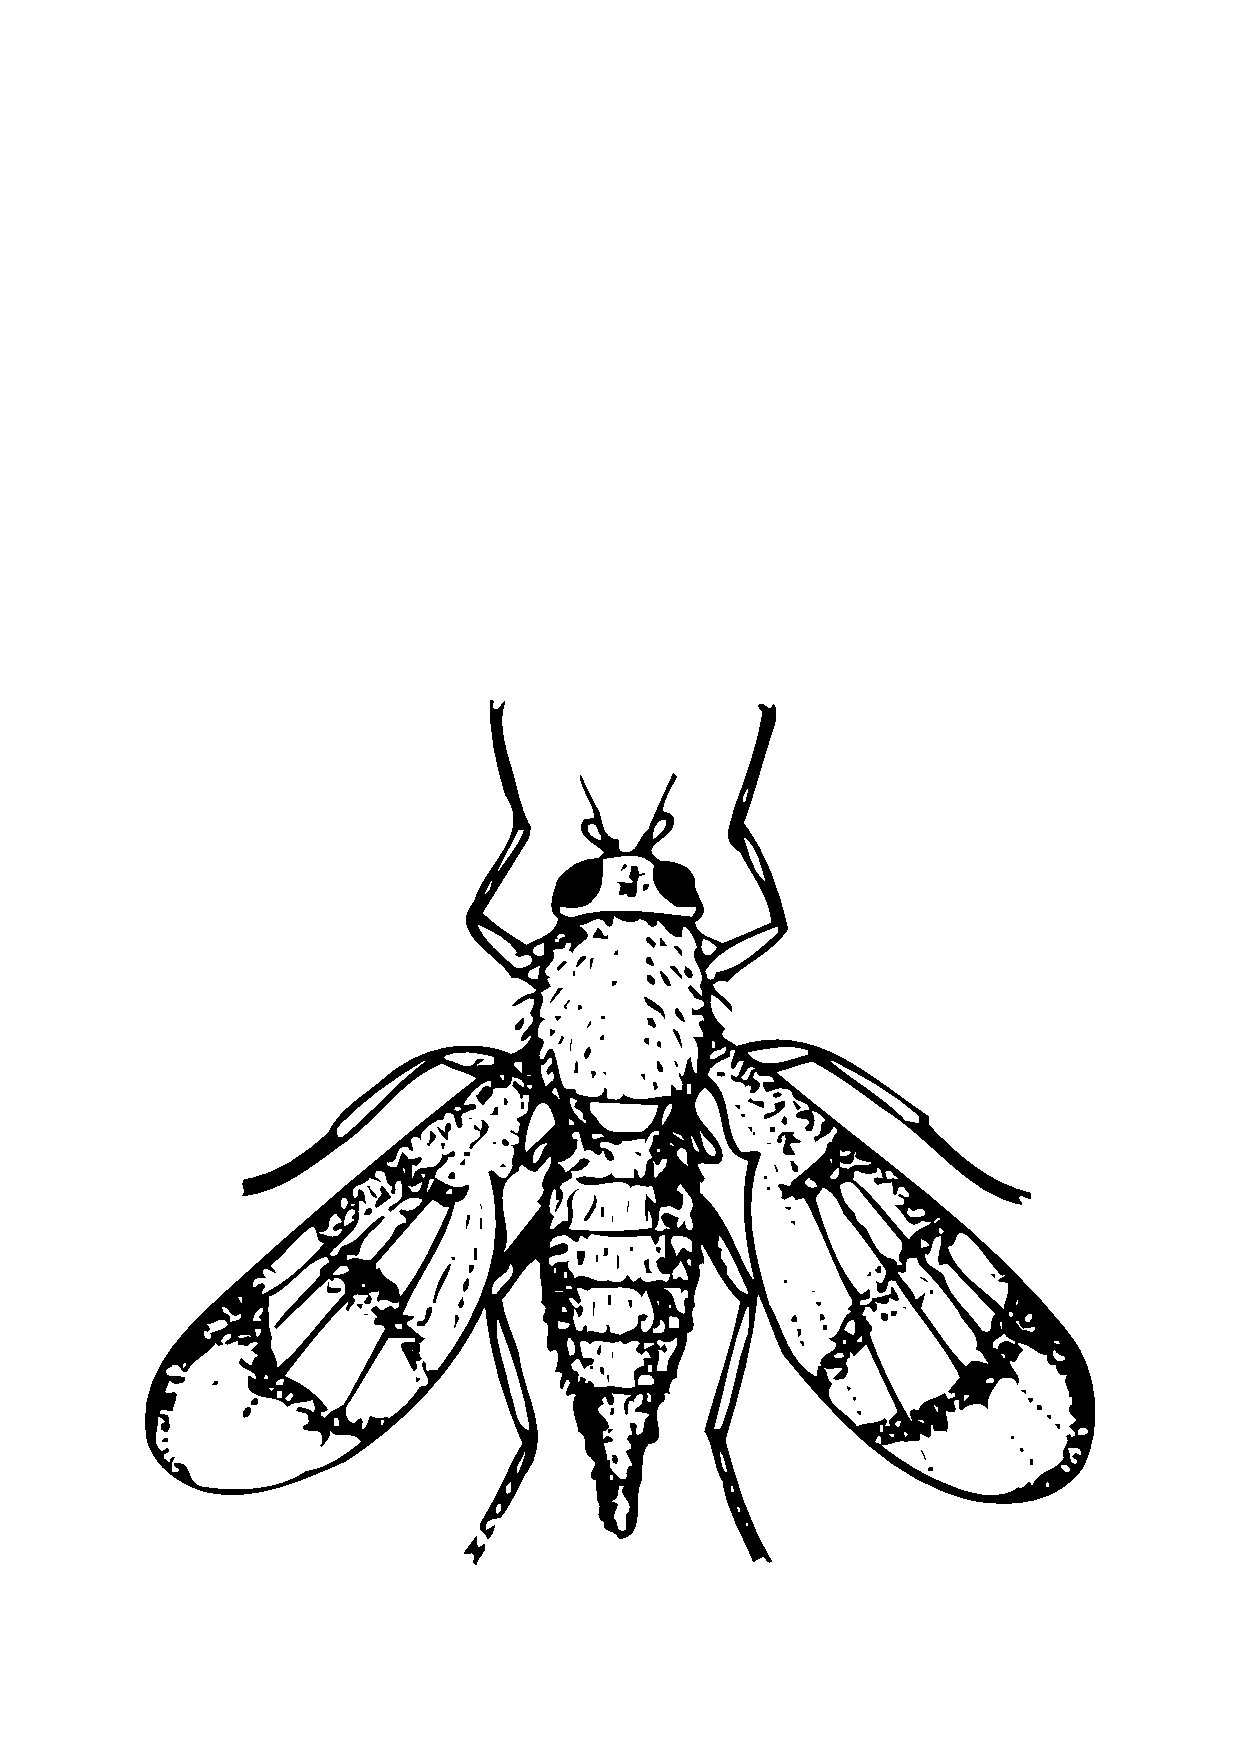
\includegraphics[width=.475\textwidth]{insect1}

\vfill

\usepicture[angle=180,origin=c]{ps:A}
\hfill
\usepicture[width=.47\textwidth]{ps:B}

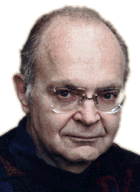
\includegraphics[width=.475\textwidth,frame=false,
  namefont={\Huge\itshape}]{knuth}
\hfill
\usepicture[angle=45,origin=bl,width=.475\textwidth,innerframe]{1}%

\vfill

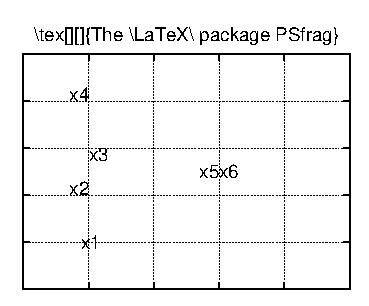
\includegraphics[width=.47\textwidth]{psf-demo}
\hfill
\begin{psfrags}
  \psfragscanon
  \psfrag{x1}[br][  ]{\LaTeX} \psfrag{x2}[br][br]{\LaTeX}
  \psfrag{x3}[br][tl]{\LaTeX} \psfrag{x4}[br][Br]{\LaTeX}
  \psfrag{x5}[Br][ r][1.15][45]{\Huge\LaTeX}
  \psfrag{x6}[tl][ l][1.15][45]{\Huge\LaTeX}
  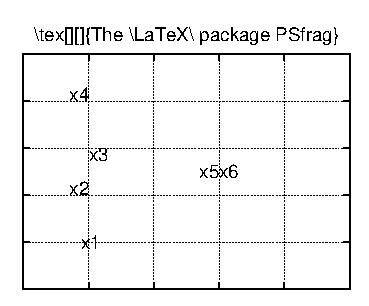
\includegraphics[width=.47\textwidth]{psf-demo}
\end{psfrags}

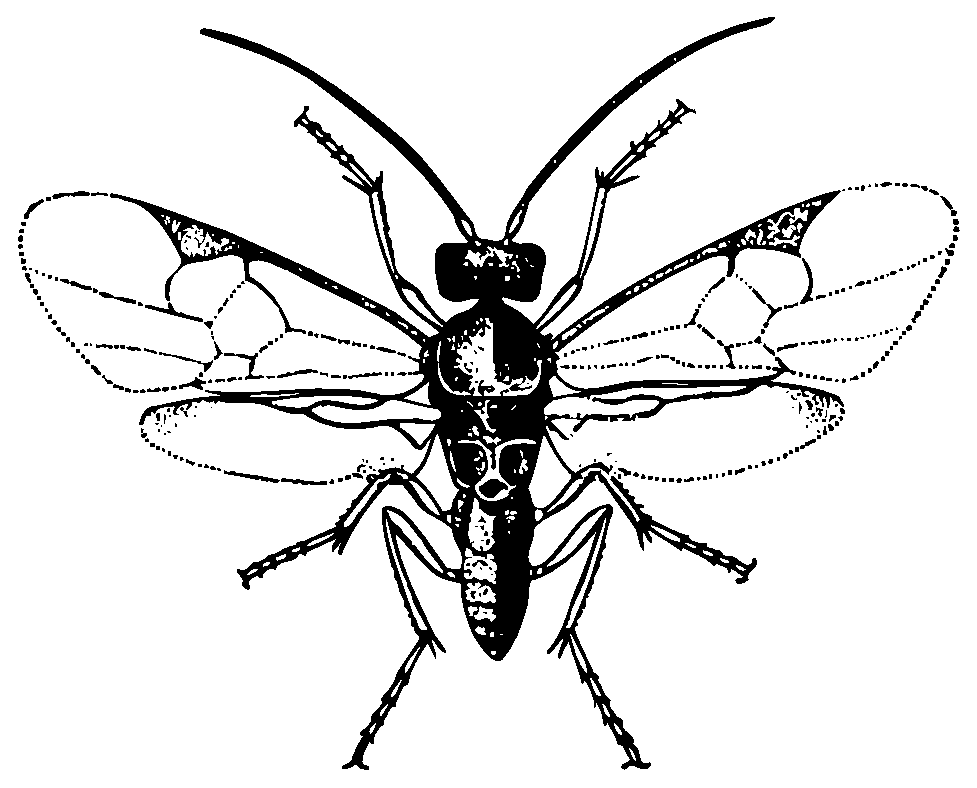
\includegraphics[width=\textwidth,showname=false,frame=false]{insect15}

\bigskip

\Large

\begin{equation}
  \sigma(t)=\frac{1}{\sqrt{2\pi}}
  \int^t_0 e^{-x^2/2} dx
\end{equation}

\clearpage

\setkeys{Gin}{showname=false,frame=false}%

{ \Huge \renewcommand*\arraystretch{1.5}

  \noindent
  \begin{tabularx}{\textwidth}{|@{}>{\centering}X@{}|} \hline

  \psframebox*[fillcolor=green,framearc=.6]{HUGO}\BASEMARKER
  \fbox{\BASEMARKER GUSTAV}  \tabularnewline

  \begin{postscript}
  \psframebox*[fillcolor=green,framearc=.6]{HUGO}\BASEMARKER
  \fbox{\BASEMARKER GUSTAV}
  \end{postscript}           \tabularnewline \hline

  \end{tabularx}

}

\bigskip

\definecolor{pink}{rgb}{1, .75, .8}
\renewcommand\psedge{\nccurve}
\newcommand{\Female}[2][]{{\psset{linecolor=pink}\TR[#1]{\emph{#2}}}}
\newcommand{\Male}[2][]{{\psset{linecolor=blue}\TR[#1]{#2}}}

\psset{nodesep=2pt,angleA=90,angleB=-90}

{ \footnotesize

   %% From: The \LaTeX\ Graphics Companion; first release.
   \pstree[treemode=U]{\Female{{\bfseries Matilde}}}{%
     \pstree{\Male{Sebastian}}{%
       \pstree{\Male[name=P]{Philip}}{\Male{Frederick}\Female{Ethel}}
       \pstree{\Female[name=W]{Mary}}{\Male{Lionel}\Female{Agnes}}}
     \pstree{\Female{Leonor}}{%
       \pstree{\Male[name=R]{Ra\'ul}}{\Male{Joaquim}\Female{J\'ulia}}
       \pstree{\Female[name=A]{Am\'elia}}{\Male{\'Alvaro}\Female{Augusta}}}
   }

  \iffalse  % --> Cannot work outside of a special environment!
  \psset{linecolor=green,doubleline=true,linestyle=dotted}
  \ncline{P}{W}\nbput{1940}
  \ncline{R}{A}\nbput{1954}
  \fi
}

\bigskip

\psset{arrows=->,fillcolor=white,fillstyle=solid}

\footnotesize

\newcommand{\Show}[1]{\psshadowbox{#1}}

\begin{psmatrix}[mnode=r,ref=t,unit=.3]
  \psframebox[linestyle=none,framesep=.75]{%
    \begin{psmatrix}[name=A,ref=c]
      \Show{Stakeholder}
    \end{psmatrix}} &
  \psframebox[fillstyle=solid,fillcolor=pink,framesep=.95]{%
    \rule{1cm}{0pt}
    \begin{psmatrix}[ref=c]
      [name=B]\Show{Goal} & \Show{Criteria}\\
              \Show{Sub-goal} & \Show{Justification}
      \ncline{1,1}{1,2}
      \ncline{1,1}{2,2}
      \ncline{1,1}{2,1}\tlput{Strategy}
      \ncline{2,1}{2,2}
    \end{psmatrix}}
  \ncline[angleB=180]{A}{B}\naput[npos=.7]{Model}
\end{psmatrix}

\begin{postscript}[angle=90,height=\textheight,frame=false]

\pstree[treemode=U]{\Female{{\bfseries Matilde}}}{%
  \pstree{\Male{Sebastian}}{%
    \pstree{\Male[name=P]{Philip}}{\Male{Frederick}\Female{Ethel}}
    \pstree{\Female[name=W]{Mary}}{\Male{Lionel}\Female{Agnes}}}
  \pstree{\Female{Leonor}}{
  \pstree{\Male[name=R]{Ra\'ul}}{\Male{Joaquim}\Female{J\'ulia}}
  \pstree{\Female[name=A]{Am\'elia}}{\Male{\'Alvaro}\Female{Augusta}}}
}

\psset{linecolor=green,doubleline=true,linestyle=dotted}
\ncline{P}{W}\nbput{1940}
\ncline{R}{A}\nbput{1954}

\end{postscript}

\bigskip

\psset{arrows=-}

\begin{displaymath}
  \bordermatrix{%
  & A            & B & C\cr
  & \rnode{D}{D} & E & \rnode{F}{F}\cr
  & G            & H & I\cr
  & \rnode{J}{J} & K & M
  }
  \ncline[nodesep=-1em,linecolor=red]{D}{F}
  \ncline[nodesep=-1em,linecolor=red]{D}{J}
\end{displaymath}

\bigskip

\mytree

\bigskip

\mymatrix

\end{document}
\endinput
%%
%% End of file `pst-pdf-example2.tex'.
